\newpage
\section{Materials and Methods}
\label{sec:Approach}

\subsection{General Problem Formulation}
\label{sec:Approach_GPF}
The general idea behind \ac{TAD} is that a high-dimensional input (e.g. a
high-resoluted or colored image) is transformed in a low-dimensional space so
that it first can be reconstructed as good as possible and second still is
human-understandable in lower dimensional space. Besides, both transformations
should be computationally efficient, so that an optimal trade-off between
network complexity (efficiency) and reconstruction capabailites is met.

\begin{figure}[!htbp]
	\centering
	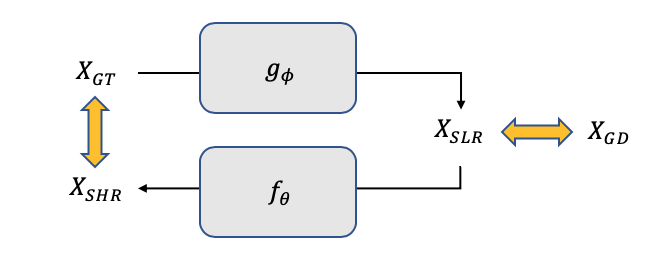
\includegraphics[width=10cm]{figures/problem}
	\caption{General \ac{TAD} problem formulation.}
  \label{fig:problem}
\end{figure}

With $g_\phi$ the downscaling and $f_\theta$ the upscaling function, $X_{GT}$
the groundtruth (input) as well as $X_{SLR}$, $X_{SHR}$ its low- and high-
dimensional representation, the \ac{TAD} problem can be formulated as combined
optimization problem constraining both the low-dimensional representation
(readibility) as well as the high-dimensional reconstruction (accuracy).
hile the second constraint can be easily formulated using the input image
$X_{GT}$ as groundtruth the first constraint is more vague and hard to quantify.
Therefore, it is assumed that the optimal latent space encoding
is similar to a trivial low-dimensional representation like a (bilinearly)
interpolated or grayscale image. As further described in
\mysecref{sec:Approach_TS} $X_{SLR}$ is thereby not derived from scratch but
builds up on the guidance image in the training procedure so that both
optimization problems can be solved more independently than learning both
$X_{SLR}$ and $X_{SHR}$ from scratch and typically the first optimization
problem (readibility of $X_{SLR}$) is easier to solve for the model.

\subsection{Autoencoder Network Design}
\label{sec:Approach_AND}
As no groundtruth for the low resolution image is available, since \ac{TAD}
poses requirements for both the down- and upscaling and because it has proven
to work for the \ac{TAD} problem in previous works an autoencoder design
is used.

\begin{figure}[!htbp]
	\centering
	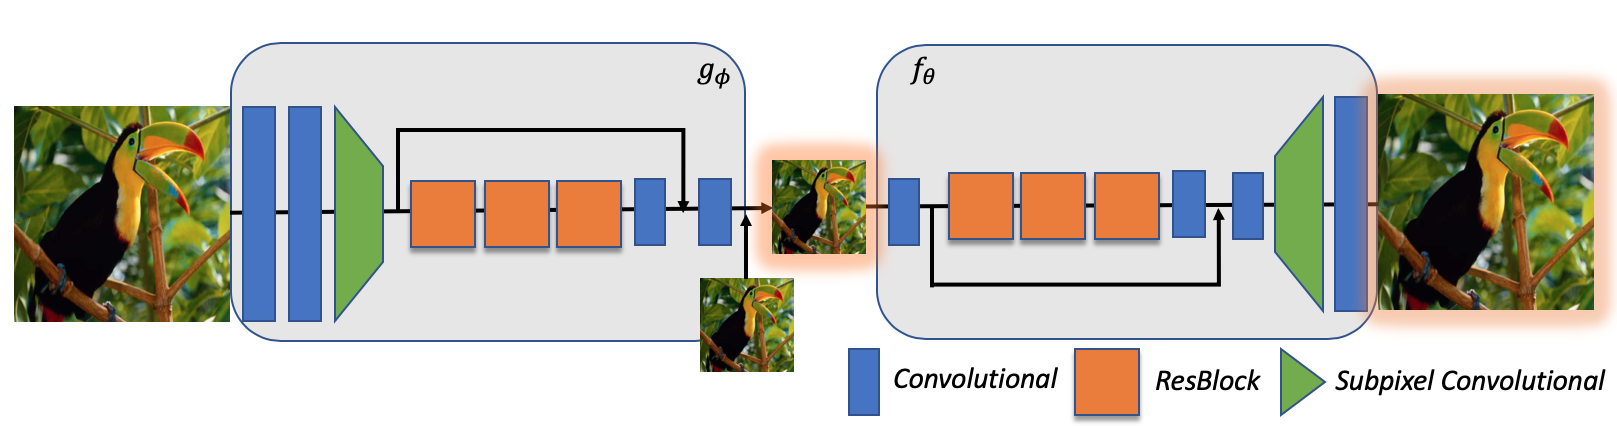
\includegraphics[width=14cm]{figures/architecture}
	\caption{Example architecture of the \ac{TAD} autoencoder network
  design for \ac{SISR} task.}
  \label{fig:architecture}
\end{figure}

The autoencoder should be able to handle an input image of general size, it
should be runtime-efficient, store as much information as possible while
downscaling as well as end-to-end and efficiently trainable.
Therefore a convolutional-only, reasonable shallow network design is used. To
avoid the loss of information during downscaling instead of pooling operations
subpixel convolutional layers are employed. Furthermore, in order to enable
efficient training and circumvent vanishing gradient problems (especially for
larger networks that were tested) next to direct forward passes ResNet
(\cite{DRLFIR}) like \textit{Resblocks} are used, which are structured as

$$Resblock(x) = x + Conv2D(ReLU(Conv2D(x)))$$

Since this network design does not continuously downscale the input but
applies pixel shuffeling to downscale while all other layers do not alter their
inputs shape, the networks also is easily adaptable to design changes, which
simplifies the architecture optimization process.

\subsection{Loss Function}
\label{sec:Approach_LF}
The loss function $L$ consists of two parts, representing both optimization
problems introduced in \mysecref{sec:Approach_GPF}. The first one, $L_{TASK}$, is
task-dependent and states the difference between the decoders output $X_{SHR}$
and the desired output $X_{GT}$, e.g. the original \ac{HR} in the \ac{SISR} task.

$$L_{TASK} = L1(X_{GT}, X_{SHR})$$

The second part, $L_{LATENT}$, encodes the human-readibility of the low-dimensional
representation. So $L_{LATENT}$ is the distance between the interpolated guidance
image $X_{GD}$ and the actual encoding $X_{SLR}$:

$$L_{LATENT} = \begin{cases}
L1(X_{GD}, X_{SLR}) & \text{if } ||L1/d_{max}|| \geq \epsilon
\\ 0.0 & \text{otherwise}
\end{cases}$$

with $||L1/d_{max}||$ being the $L1(X_{GD}, X_{SLR})$ loss normalized
by the maximal deviation between $X_{GD}$ and $X_{SLR}$. Hence, $L_{LATENT}$
is zero in an $l1$-ball around the guidance image, ensuring that \ac{SLR} is
close to the guidance image but also helps to prevent overfitting to the trivial
solution $X_{GD} = X_{SLR} \Leftrightarrow g_\phi = 0$. As shown in
\mychapterref{sec:ExperimentsandResults} introducing an $l1$-ball also improves
the model's robustness against perturbations.
\newline
The overall loss function is a weighted sum of both of the loss function
introduced above. The relative weight $(\alpha, \beta)$ is of large importance
for the trade-off between the readibility requirement and the performance of the
model's upscaling part (super resolution, colorization). However, as described
above the readibility requirement is less strict so that typically
$\alpha >> \beta$.

$$L = \alpha L_{TASK} + \beta L_{LATENT}$$

\subsection{Training Specifications}
\label{sec:Approach_TS}
Even if a guidance image is part of the loss function learning both the low-
and high-dimensional representation from scratch poses a combined optimization
problem which usually is very hard to solve. To ensure (faster) convergence,
therefore in the beginning of the training procedure the guidance image is
added to the encoder's output. This improves both the convergence rate of
$X_{SLR}$ and $X_{SHR}$, especially in the beginning of the training procedure,
since merely a difference between the interpolated representation and the more
optimal encoding has the be derived and the down- and upscaling can be learnt
more independently since the lower dimensional representation is always
guaranteed to be useful for upscaling.

\begin{figure}[!htbp]
	\centering
	
\includegraphics[width=10cm]{figures/cvl}
	\caption{Loss curve without adding guidance image (left) and with
  adding guidance image (right) while training.}
  \label{fig:loss_w_wo_adding_guidance}
\end{figure}

\subsection{Implementation}
\label{sec:Approach_IMP}
The project was implemented in Python 3, using the PyTorch deep learning
framework. Although some ideas from Kim et al. \cite{TAID} were adopted as
described above the pipeline had to be re-implemented from scratch and
re-validated since neither code nor any pretrained model have been
available publically (nor upon request). As PyTorch merely supports
subpixel convolutional layers, their inverse transformation was implemented as
well. During program development it was paid attention to generality and
commutability in order to efficiently test a variety of different models and
datasets as well as guarantee comparability of different approaches. 

% The objectives of the ``Materials and Methods'' section are the following:
% \begin{itemize}
%  \item \textit{What are tools and methods you used?} Introduce the environment, in which your work has taken place - this can be a software package, a device or a system description. Make sure sufficiently detailed descriptions of the algorithms and concepts (e.g. math) you used shall be placed here.
%  \item \textit{What is your work?} Describe (perhaps in a separate section) the key component of your work, e.g. an algorithm or software framework you have developed.
% \end{itemize}
